% !TEX options=--shell-escape
\documentclass [12pt]{article} 
\usepackage {amsmath}
\usepackage {amsthm}
\usepackage {amssymb}
\usepackage {graphicx} 
\usepackage {float}
\usepackage {multirow}
\usepackage {xcolor}
\usepackage {algorithmic}
\usepackage [ruled,vlined,commentsnumbered,titlenotnumbered]{algorithm2e} \usepackage {array} 
\usepackage {booktabs} 
\usepackage {url} 
\usepackage {parskip} 
\usepackage [margin=1in]{geometry} 
\usepackage [T1]{fontenc} 
\usepackage {cmbright} 
\usepackage [many]{tcolorbox} 
\usepackage [colorlinks = true,
            linkcolor = blue,
            urlcolor  = blue,
            citecolor = blue,
            anchorcolor = blue]{hyperref} 
\usepackage {enumitem} 
\usepackage {xparse} 
\usepackage {verbatim}
\usepackage{listings}
\usepackage{xcolor}
\usepackage{csquotes}
\usepackage[cache=false]{minted}
\usepackage{mdframed}
\usepackage{tikz}
\usetikzlibrary{shapes.symbols}
\newtheorem{theorem}{Theorem}

\DeclareTColorBox {Solution}{}{breakable, title={Solution}}
\DeclareTColorBox {Solution*}{}{breakable, title={Solution (provided)}}
\DeclareTColorBox {Instruction}{}{boxrule=0pt, boxsep=0pt, left=0.5em, right=0.5em, top=0.5em, bottom=0.5em, arc=0pt, toprule=1pt, bottomrule=1pt}
\DeclareDocumentCommand {\Expecting }{+m}{\textbf {[We are expecting:} #1\textbf {]}}
\DeclareDocumentCommand {\Points }{m}{\textbf {(#1 pt.)}} 
\newcommand {\hint }[1]{\noindent {[\textbf {HINT:} \em #1 \em ]}} \newcommand {\pts }[1]{\textbf {(#1 pt.)}} 

\begin{document} 

{\LARGE \textbf {COMP 285 (NC A\&T, Spr `22)}\hfill \textbf {Weekly Quiz 4} } 

\begin{Instruction}

\paragraph{Reporting Issues} If you find any issues with the solutions, reach out to Chi Wang (author) or Luis Perez (reviewer).

\end{Instruction}


\section{} Assume you have a function called 3Sort that takes as input an array of size 3 of comparable objects and returns them in sorted order. You want to sort an array of size $n \geq 3$ objects only using callsto 3Sort. How many function calls of 3Sort are required to sort an array of size $n$? Choose the asymptotically largest applicable lower bound.

\begin{Solution}
$\Omega(n \log n)$
\paragraph{} 
It's just similar with sorting the array directly (Using a Comparison Sort with Merge Sort). The only difference is that we compare 3 elements each time instead of 2.
\paragraph{} 


\end{Solution}


\section{} I claim to have a data structures that can store comparable objects and supports the following operations: 
\begin{enumerate}
    \item insert new objects in $O(1)$ time per insertion
    \item remove objects in $O(1)$ time per removal
    \item return the smallest object in the data structures in $O(1)$ time. 
\end{enumerate}

Is it possible to have such a data structure? (Hint: Recall that sorting $n$ comparable elements must take at least $O(n \log n)$ time. Can you sort faster if the data structure I described above exists?)

\begin{Solution}
Impossible
\paragraph{} 
It is possible to insert/remove objects in average O(1) time, however, it's impossible to return the smallest object in O(1) time. If we could find the smallest element is O(1) time, then the whole array could be sort in O(n) time.

Recall that sorting $n$ comparable elements must take at least $O(n \log n)$.
\end{Solution}


\section{} Assume you have an array $A$ of size n with positive integer element with all elements in the range [1, $n^3$).  What is the runtime of Radix Sort using base 10 run on A? 

\textbf{Hint:} The runtime of radix sort is $O(d (n+r))$, where n is the size of your input array, r is the number of buckets, and d is the number of digits.

\begin{Solution}
$\Theta(nlogn)$
\paragraph{} 
$d = \lfloor log_10(n) \rfloor + 1$, so time $= O(nd) = O(n log (n))$.

\end{Solution}


\section{} The runtime of Radix Sort is $O(d(n+r))$ where $d$ is the number of digits in our base, $n$ is the number of elements we're sorting, and $r$ is the number of buckets we're using to sort (our base). When sorting integers, what is a ``good'' choice of $r$?

\begin{Solution}
$n$
\paragraph{}
Compared with 2, 10, $n^2$ this gives the best running time.

\end{Solution}


\section{} Which of the following describes the height of a red-black tree on $n$ nodes?

\begin{Solution}
\begin{itemize}
    \item $\Theta(\log n)$ because a red-black tree is balanced, which means its height is $\Theta(\log n)$.
    \item $O(\log n)$ because if the height is $\Theta(\log n)$ then it is both an upper and lower bound.
    \item $\Omega(\log n)$ because if the height is $\Theta(\log n)$ then it is both an upper and lower bound.
\end{itemize}
\end{Solution}


\section{} If the length of a path from the root of a red-black tree to one of the leaf NIL nodes is 100, what could be the length of another path from the root to some other NIL node?

\begin{Solution}
180
\paragraph{}
Compared with 30 and 45, both of which are far too small. Even if they consist of all black-nodes, the longest other path could be at most 60 and 90 (respectively).

Red-Black Trees always have height at most $2*\log(n+1)$, since path can be at most twice as long another if we pad it with red nodes.
\end{Solution}


\section{} What is the worst-case runtime of operations INSERT/DELETE/SEARCH on a red-black tree storing $n$ nodes?

\begin{Solution}
$$\Theta(\log n)$$

As with general Binary Search Trees, all operations are O(height). So all operations with RBTrees are $O(\log(n))$.
\end{Solution}


\section{} Hash tables with universal hash families guarantee an expected runtime of $O(1)$ for the INSERT,SEARCH, and DELETE operations. 

\begin{Solution}
True. This is the definition of a hash table.
\end{Solution}


\section{} Suppose that the nodes A,B,C in a binary search tree are arranged as follows. (The tree has no duplicate nodes.). What must be true?
\begin{figure}[H]
    \centering
    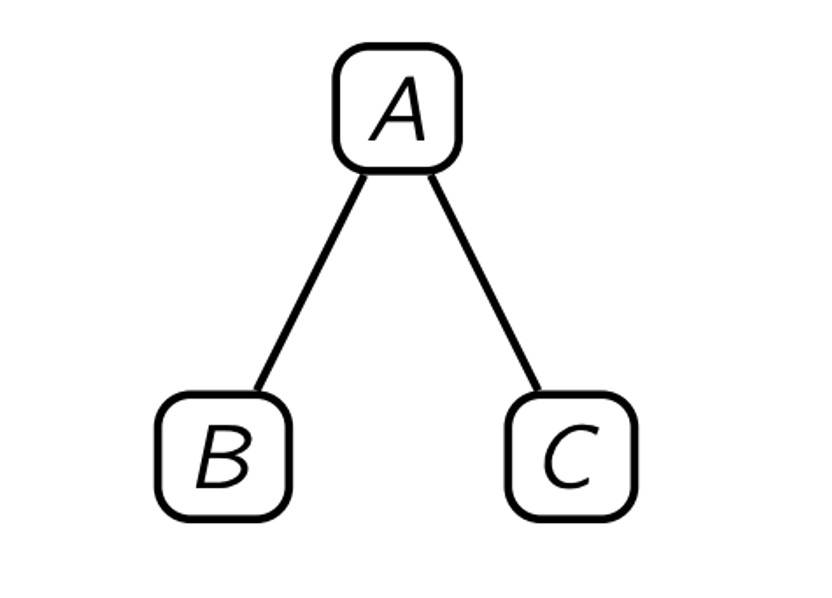
\includegraphics[scale=0.5]{pic1.png} 
    \label{fig:my_label}
\end{figure}

\begin{Solution}
$$B < A < C$$
By definition of the binary search tree.
\end{Solution}


\section{} Is the following a valid red-black tree? 
\begin{figure}[H]
    \centering
    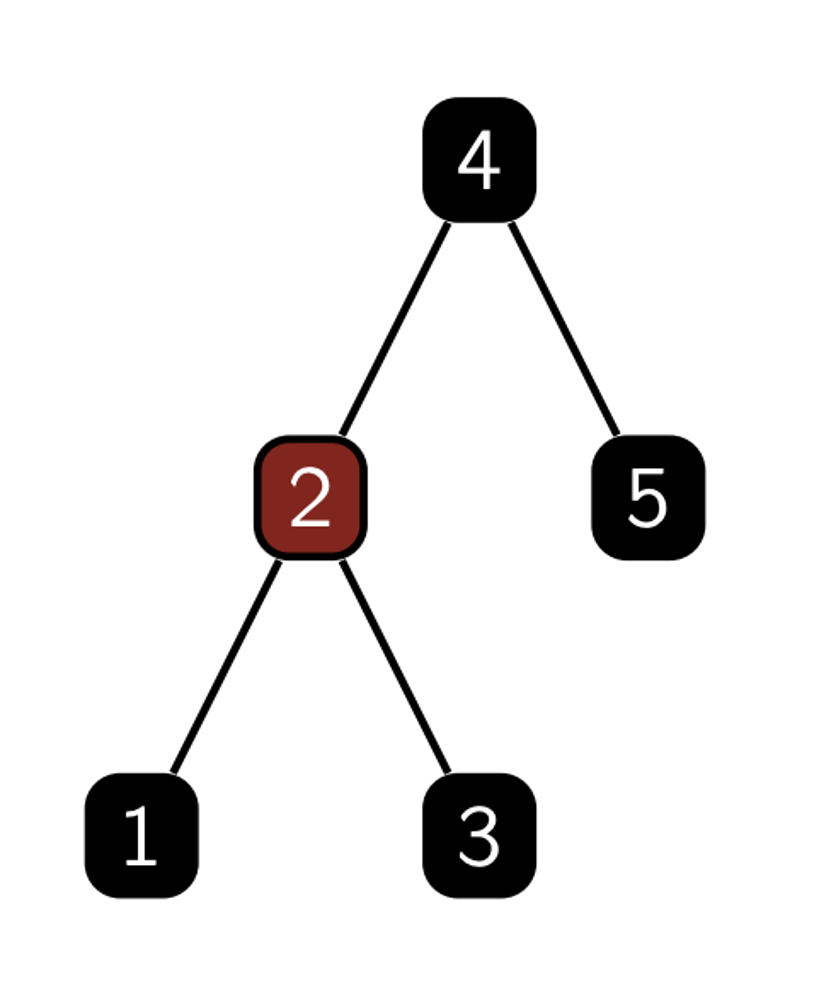
\includegraphics[scale=0.5]{pic2.png} 
    \label{fig:my_label}
\end{figure}

\begin{Solution}
Yes
\paragraph{}
By definition of the red-black tree.
\end{Solution}


















\end{document} 